\section{Medical Image Routing Model}
This section presents the proposed medical image routing model employed in the system and discusses the motivation behind the model, its problem formulation, and finally its architecture. This model serves as the decision-making unit of the system, where the destination of each input image is determined and forwarded thereafter.

\subsection{Motivation}
The increasing use of deep learning in medical image analysis has enabled the development of highly specialized models for tasks such as disease detection and diagnosis. In the context of lung cancer detection, chest X-ray and computed tomography (CT) images provide complementary diagnostic information and often require different processing pipelines and model architectures. While chest X-rays offer a low-cost and widely accessible imaging modality for preliminary screening, CT scans provide detailed cross-sectional information that supports more comprehensive assessment of lung abnormalities.

However, in real-world deployment scenarios, diagnostic systems are often exposed to heterogeneous image inputs originating from different imaging modalities, anatomical regions, or acquisition protocols. Applying a modality-specific diagnostic model to an inappropriate image type may lead to unreliable predictions and compromise the robustness and safety of the overall system. Consequently, there is a need for an initial classification mechanism capable of identifying the nature of incoming medical images before further analysis is performed.

This section introduces a medical image classification model designed to function as an image routing component within a larger lung cancer diagnostic pipeline. The model distinguishes between chest X-ray images, chest CT scan images, and an additional out-of-distribution category referred to as “Other.” By incorporating this third category, the system is able to explicitly handle images that do not belong to the intended diagnostic classes, thereby reducing the risk of misclassification and improving overall system reliability. Once classified, chest X-ray and CT scan images are forwarded to their corresponding lung cancer diagnostic models, while out-of-distribution images are rejected from further analysis. The following subsections present the motivation for this approach, formally define the classification problem, and describe the model architecture employed.

\subsection{Problem Statement}

The goal of this work is to develop an automated medical image classification model capable of identifying the type of an input image and routing it to the appropriate downstream analysis. The task is formulated as a three-class classification problem, where each input image \(X \in \mathbb{R}^{224 \times 224 \times 3}\) must be assigned to one of three categories: chest X-ray images (\(0\)), chest CT scan images (\(1\)), or out-of-distribution images labeled as \emph{Other} (\(2\)). This multi-class formulation ensures that irrelevant or ambiguous inputs are explicitly handled, improving system safety and reducing the risk of inappropriate downstream processing.

The model is designed to output a probability distribution \(\mathbf{p} = [p_0, p_1, p_2]\) over the three classes, where \(p_k = P(y = k \mid X)\) and \(\sum_{k=0}^{2} p_k = 1\). The predicted class is obtained by selecting the class with the highest probability, \(\hat{y} = \arg\max_{k} p_k\). Images classified as chest X-rays are forwarded to the X-ray-based lung cancer detection model, while images classified as CT scans are routed to the CT-based lung cancer detection model. By incorporating the \emph{Other} category, the model avoids forcing all inputs into diagnostic categories and can robustly separate images outside the target distribution, laying a solid foundation for safe integration within a larger medical image analysis pipeline.

\subsection{Model Architecture}

The proposed medical image classification model is designed using a transfer learning approach based on the ResNet50 convolutional neural network. The architecture follows a structured pipeline consisting of input preprocessing, deep feature extraction, feature aggregation, and final classification. This modular design allows the model to benefit from representations learned on large-scale image datasets while adapting effectively to the target medical imaging task. An overview of the complete classification pipeline is illustrated in Figure~\ref{fig:overall_architecture}.

\begin{figure}[h]
	\centering
	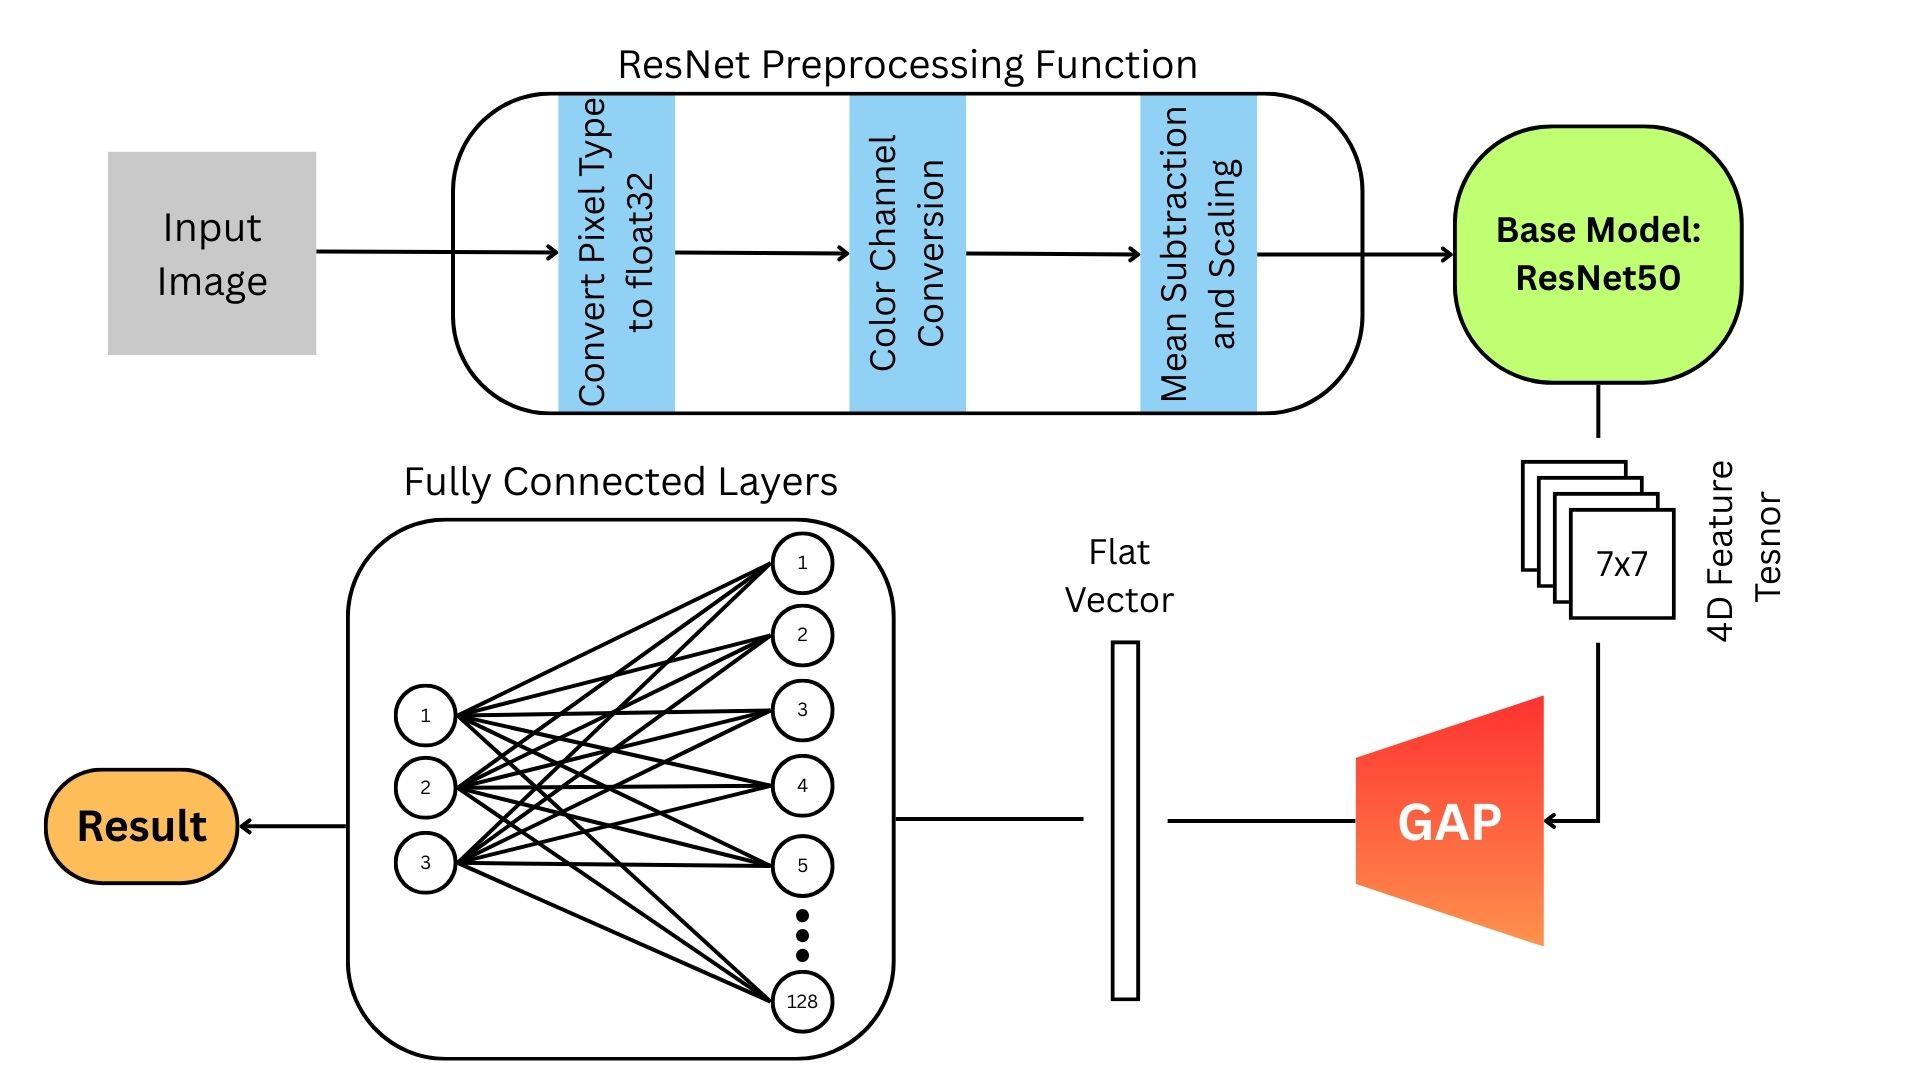
\includegraphics[width=0.95\linewidth]{assets/router-architecture.jpg}
	\caption{Overall architecture of the proposed medical image routing model.}
	\label{fig:overall_architecture}
\end{figure}

The input to the model is a medical image \(X \in \mathbb{R}^{224 \times 224 \times 3}\), resized to a fixed spatial resolution and represented in RGB color space. Prior to being processed by the pretrained network, the image undergoes a preprocessing step to ensure compatibility with the ResNet50 weights. This step mirrors the preprocessing applied during the original ImageNet training of ResNet50 and is essential for effective transfer learning. Specifically, the input image is first converted to floating-point representation, its color channels are reordered from RGB to BGR, and a fixed channel-wise mean is subtracted. Let \(X_{rgb}\) denote the raw input image; the preprocessed image \(X_{prep}\) is obtained as \(X_{prep} = \mathrm{BGR}(X_{rgb}) - \mu\), where \(\mu = [103.939, 116.779, 123.68]\) represents the ImageNet mean for the blue, green, and red channels, respectively. This operation centers the input distribution around zero and aligns it with the statistical properties expected by the pretrained backbone.

Following preprocessing, the image is passed through the ResNet50 network with its original classification layers removed. In this configuration, ResNet50 functions as a fully convolutional feature extractor. For an input tensor of shape \((224, 224, 3)\), the output of the backbone is a high-dimensional feature map of shape \((7, 7, 2048)\). This tensor contains 2048 feature channels, each encoding abstract visual patterns such as anatomical structures, textures, and modality-specific characteristics while preserving coarse spatial relationships within the image. For a detailed discussion of the ResNet50 model architecture, refer to Subsection~\ref{subsec:resnet50-arch}.

To transform the spatial feature maps into a compact representation suitable for classification, a global average pooling operation is applied to the output of the ResNet50 backbone. This operation computes the average activation of each feature channel across the spatial dimensions, effectively summarizing the presence of each learned feature over the entire image. Given a feature map \(F \in \mathbb{R}^{7 \times 7 \times 2048}\), the pooled feature vector \(z \in \mathbb{R}^{2048}\) is computed such that each element \(z_k\) corresponds to the mean of the activations in channel \(k\), i.e.
\begin{equation*}
	z_k = \frac{1}{7 \times 7} \sum_{i=1}^{7} \sum_{j=1}^{7} F_{i,j,k}
\end{equation*}
This operation reduces the tensor shape from \((7, 7, 2048)\) to \((2048)\) while significantly lowering the number of parameters required in subsequent layers and improving generalization.

The resulting feature vector is then passed to a task-specific classification head composed of fully connected layers. These layers learn discriminative combinations of the extracted features and map them to the target class space. The final layer applies a softmax activation function, producing a probability distribution \(\mathbf{p} = [p_0, p_1, p_2]\), where each component represents the predicted probability of the image belonging to the chest X-ray class, chest CT scan class, or the out-of-distribution \emph{Other} class. The predicted label is obtained as \(\hat{y} = \arg\max_k p_k\).